\documentclass[tikz,border=6pt]{standalone}
\usepackage{amsmath}
\usetikzlibrary{arrows.meta,positioning,fit}
\begin{document}
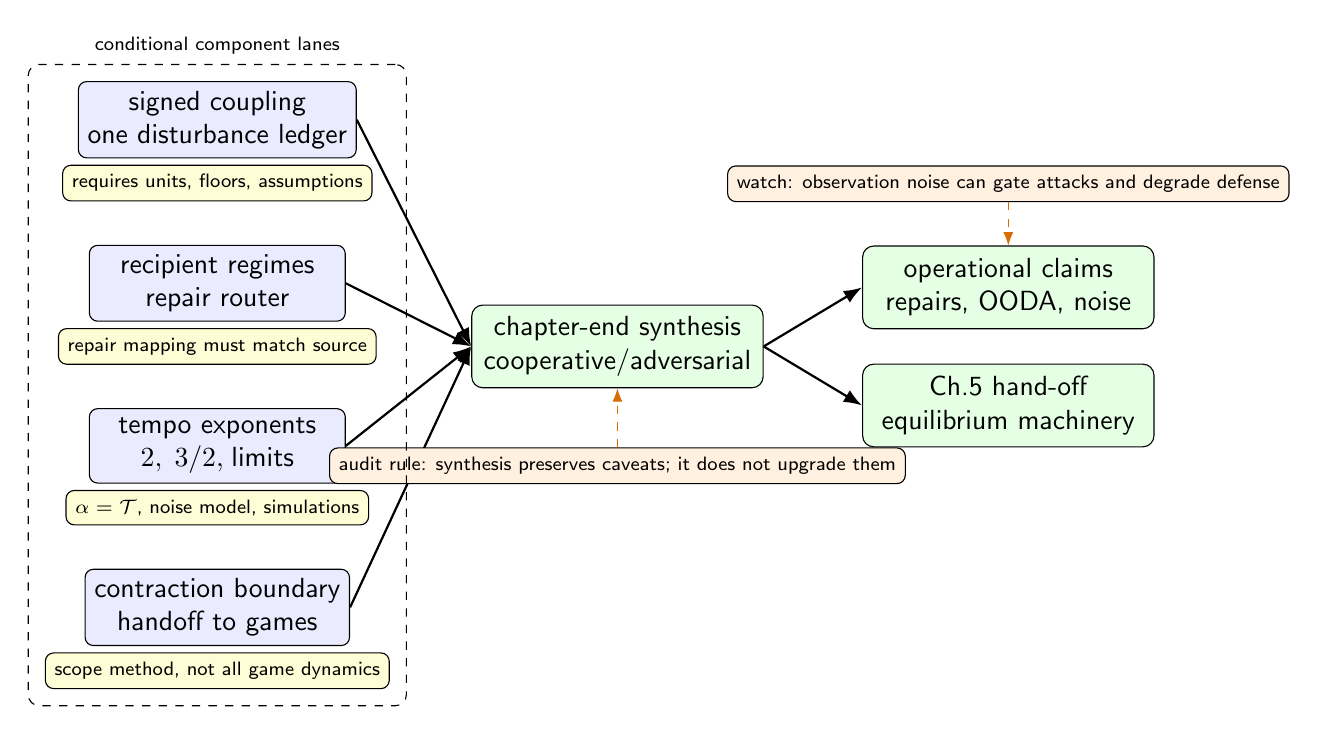
\begin{tikzpicture}[
  font=\sffamily,
  >=Latex,
  lane/.style={draw, rounded corners=3pt, fill=blue!8, align=center, minimum width=3.25cm, minimum height=0.82cm},
  caveat/.style={draw, rounded corners=3pt, fill=yellow!16, align=center, font=\sffamily\scriptsize, minimum width=3.25cm},
  synth/.style={draw, rounded corners=4pt, fill=green!10, align=center, minimum width=3.7cm, minimum height=1.05cm},
  warn/.style={draw, rounded corners=3pt, fill=orange!12, align=center, font=\sffamily\scriptsize}
]

\node[lane] (signed) {signed coupling\\one disturbance ledger};
\node[caveat, below=0.08cm of signed] (signedc) {requires units, floors, assumptions};

\node[lane, below=0.55cm of signedc] (regime) {recipient regimes\\repair router};
\node[caveat, below=0.08cm of regime] (regimec) {repair mapping must match source};

\node[lane, below=0.55cm of regimec] (tempo) {tempo exponents\\$2,\;3/2,\;$limits};
\node[caveat, below=0.08cm of tempo] (tempoc) {$\alpha=\mathcal T$, noise model, simulations};

\node[lane, below=0.55cm of tempoc] (contract) {contraction boundary\\handoff to games};
\node[caveat, below=0.08cm of contract] (contractc) {scope method, not all game dynamics};

\node[synth, right=1.2cm of regimec] (chapter) {chapter-end synthesis\\cooperative/adversarial};
\node[synth, right=1.25cm of chapter, yshift=0.75cm] (claims) {operational claims\\repairs, OODA, noise};
\node[synth, right=1.25cm of chapter, yshift=-0.75cm] (handoff) {Ch.5 hand-off\\equilibrium machinery};

\draw[->, thick] (signed.east) -- (chapter.west);
\draw[->, thick] (regime.east) -- (chapter.west);
\draw[->, thick] (tempo.east) -- (chapter.west);
\draw[->, thick] (contract.east) -- (chapter.west);
\draw[->, thick] (chapter.east) -- (claims.west);
\draw[->, thick] (chapter.east) -- (handoff.west);

\node[warn, below=0.75cm of chapter, minimum width=4.2cm] (status)
  {audit rule: synthesis preserves caveats; it does not upgrade them};
\draw[->, dashed, orange!85!black] (status.north) -- (chapter.south);

\node[warn, above=0.55cm of claims, minimum width=4.2cm] (noise)
  {watch: observation noise can gate attacks and degrade defense};
\draw[->, dashed, orange!85!black] (noise.south) -- (claims.north);

\node[draw, dashed, rounded corners=4pt, fit=(signed) (contractc), inner sep=6pt,
      label={[font=\sffamily\scriptsize]above:conditional component lanes}] {};

\end{tikzpicture}
\end{document}
